% !Mode:: "TeX:UTF-8"
%% 请使用 XeLaTeX 编译本文.
% \documentclass{WHUBachelor}% 选项 forprint: 交付打印时添加, 避免彩色链接字迹打印偏淡. 即使用下一行:
 \documentclass[forprint]{MyReportTem}

\begin{document}
%%%%%%% 下面的内容, 据实填空.

\StudentNumber{201728007010000} % 填写自己的学号
\ClassNumber{66} 	%你的课程序号
\Classlabel{}	%课程的编号
\Cclassname{}	%课程的名称
\title{李磊的课程报告~\LaTeX~模板}
\Etitle{A \LaTeX~Thesis Template for lilei} % 英文题目
\author{李磊}                            % 作者名字
\Eauthor{Li Lei}            %作者英文名
\Csupervisor{王力哲\quad 教授}        %指导教师中文名、职称
\Esupervisor{Prof.~Wang Li-zhe}     %指导教师英文名、职称
\Cmajor{地图学与地理信息系统}                  % 专业中文名
\Emajor{Cartography and Geographical Information System}% 专业英文名
\Cschoolname{资源与环境学院}          % 学院名
\Eschoolname{College of Environment and Resources} %学院英文名. 
\date{二〇一七年十二月}                    % 日期, 要注意和英文日期一致!!
\Edate{Dec, 2017}                       % 英文封面日期

%-----------------------------------------------------------------------------
\pdfbookmark[0]{封面}{title}         % 封面页加到 pdf 书签
\maketitle
%英文题目,中英文摘要,以及声明信息,不需要则注释掉下一行
\frontmatter

\pagenumbering{Roman}              % 正文之前的页码用大写罗马字母编号.
%-----------------------------------------------------------------------------
%如果不需要英文题目,中英文摘要,以及声明信息,则注释掉下一行
% !Mode:: "TeX:UTF-8"

%%% 此部分需要自行填写: (1) 中文摘要及关键词 (2) 英文摘要及关键词
%%%%%%%%%%%%%%%%%%%%%%%%%%%%%
%%% -------------  英文封面 (无需改动)-------------   %%%
%%%%%%%%%%%%%%%%%%%%%%%%%%%%%
\thispagestyle{empty}
\renewcommand{\baselinestretch}{1.5}  %下文的行距
\vspace*{0.5cm}
\begin{center}
{\Large \bf BACHELOR'S DEGREE THESIS \\[1ex] OF WUHAN UNIVERSITY }
\end{center}
\vspace{2.5cm}
\begin{center}{\zihao{2} \the\Etitle \par}\end{center}

\vfill

\begin{center}
\zihao{4}
\begin{tabular}{ r l }
 School (Department): & {\sc \the\Eschoolname}\\
  Major:          &   {\sc\the\Emajor}  \\
 Candidate:      &  {\sc \the\Eauthor}      \\
 Supervisor:     &  {\sc \the\Esupervisor}
\end{tabular}

\vspace*{2cm}
\begin{center}
   \ifprint % 文档打印, 使用黑白校徽.
  
\includegraphics[height=4cm]{whu.eps}       %%  黑白的.
  \else
  
\includegraphics[height=4cm]{whulogo.eps} %%  彩色的.
  \fi
\end{center}


\zihao{-2}
%\the\Schoolname\\
{\sc Wuhan University}

\vspace*{1.0cm}

\the\Edate

\end{center}
%%% 郑重声明部分无需改动

%%%---- 郑重声明 (无需改动)------------------------------------%
\newpage
\vspace*{20pt}
\begin{center}{\ziju{0.8}\textbf{\songti\zihao{2} 郑重声明}}\end{center}
\par\vspace*{30pt}
\renewcommand{\baselinestretch}{2}

{\zihao{4}%

本人呈交的学位论文, 是在导师的指导下, 独立进行研究工作所取得的成果,
所有数据、图片资料真实可靠. 尽我所知, 除文中已经注明引用的内容外,
本学位论文的研究成果不包含他人享有著作权的内容.
对本论文所涉及的研究工作做出贡献的其他个人和集体,
均已在文中以明确的方式标明. 本学位论文的知识产权归属于培养单位.\\[2cm]

\hspace*{1cm}本人签名: $\underline{\hspace{3.5cm}}$
\hspace{2cm}日期: $\underline{\hspace{3.5cm}}$\hfill\par}
%------------------------------------------------------------------------------
\baselineskip=23pt  % 正文行距为 23 磅
%------------------------------------------------------------------------------





%%======中文摘要===========================%
\begin{cnabstract}
本文主要介绍和讨论了武汉大学本科毕业论文的~\LaTeX~模板.
指明了编译方法, 强调了公式排版的一些细节问题, 也指出了一些常见的排版错误.



\end{cnabstract}
\par
\vspace*{2em}


%%%%--  关键词 -----------------------------------------%%%%%%%%
%%%%-- 注意: 每个关键词之间用“;”分开,最后一个关键词不打标点符号
\cnkeywords{毕业论文; \LaTeX{}; 模板;  }


%%====英文摘要==========================%


\begin{enabstract}
This thesis is a study on the theory of \dots.

\end{enabstract}
\par
\vspace*{2em}

%%%%%-- Key words --------------------------------------%%%%%%%
%%%%-- 注意: 每个关键词之间用“;”分开,最后一个关键词不打标点符号
 \enkeywords{\LaTeX{};  }
    % 加入英文封面,摘要, 申明.
%==========================把目录加入到书签==============================%%%%%%
%如果不需要目录,则注释掉下两行
\pdfbookmark[0]{目录}{toc}
\tableofcontents

\mainmatter %% 以下是正文
%%%%%%%%%%%%%%%%%%%%%%%%%%%--------main matter-------%%%%%%%%%%%%%%%%%%%%%%%%%%%%%%%%%%%%
\chapter{先说重要的}
本模板基于武汉大学数学与统计学院黄正华的武汉大学本科毕业论文模板,可以在此获取原文档\url{http://aff.whu.edu.cn/huangzh/}
 \section{具体使用步骤}

 \begin{description}

  \item[Step 1]  进入 includefile 文件夹,  打开 frontmatter.tex, backmatter.tex 这两个文档,
        分别填写 (1) 中文摘要、英文摘要, (2) 致谢.(如果需要的话)

  \item[Step 2]  打开主文档 Report--template.tex, 填写题目、作者等等信息, 书写正文.

  \item[Step 3]  使用 XeLaTeX 编译. 具体见 \ref{sec-compile} 节.


\end{description}



\section{编译的方法}\label{sec-compile}

默认使用 XeLaTeX 编译, 直接生成~pdf 文件.

若另存为新文档, 请确保文档保存类型为 \verb|:UTF-8|. 当然目前很多编辑器默认文字编码为 UTF-8.
WinEdt 9.0 之后的版本都是默认保存为 UTF-8 的.


%使用~XeLaTeX 编译, 直接生成~pdf 文件.
%pdf 文件也可以反向搜索! \CJKunderwave{双击~pdf 中要修改的文字, 将直接跳转到源文件中相应位置.}
%





\section{文档类型选择}
文档类型有 2 种情形:

\begin{table}[ht]\centering
\begin{tabular}{ll}
\hline
   \verb|\documentclass{MyReportTem}|                     &  毕业论文 \\
   \verb|\documentclass[forprint]{MyReportTem}|        &  毕业论文打印版 \\
\hline
\end{tabular}
\end{table}
相关解释见下节.


\section{打印的问题}
\begin{enumerate}[i)]
%  \item  论文要求\colorbox{yellow}{单面打印}.
  \item  关于文档选项 forprint: 交付打印时, 建议加上选项 forprint, 以消除链接文字之彩色, 避免打印字迹偏淡.
  \item  打印时留意不要缩小页面或居中. 即页面放缩方式应该是``无''(Adobe Reader XI 是选择``实际大小'').
           有可能页面放缩方式默认为``适合可打印区域'', 会导致打印为原页面大小的 $97\%$.
           文字不要居中打印, 是因为考虑到装订, 左侧的空白留得稍多一点(模板已作预留).
  \item  遗留问题: 封面需要打印部重新制作.  校内打印部通常有现成的模板.
           我们自己做的封面, 打印部不一定好用.
\end{enumerate}
%如果不是彩色打印机, 请在打印时, 选择将彩色打印为黑白, 否则彩色文字打出的墨迹会偏淡.

\textbf{问}: {\kaishu 生成 PDF 文件时,不能去掉目录和文章的引用彩色方框,请问怎么解决?}

\textbf{答}: {\kaishu 方框表示超级链接, 只在电脑上看得见. 实际打印时, 是没有的. 另外, 文档类型加选项 forprint 之后, 这些框框会隐掉的. }

 \vfill

本文档更改于以下文档: \url{http://aff.whu.edu.cn/huangzh/}. 此文档是武汉大学本科毕业生论文的模板,如需使用, 请移步.

问题反馈及建议, 请联系: huangzh@whu.edu.cn.



\chapter{杂七杂八的话}

\section{Readme}

模板文件的结构, 如下表所示:
 \begin{table}[ht]\centering
\begin{tabular}{r|r|l}
	\hline\hline
	\multicolumn{2}{l|}{Bachelor-template.tex }       & 主文档. 在其中填写正文.             \\ \hline
	                                & frontmatter.tex & 郑重声明、中英文摘要.               \\ \cline{2-3}
	\raisebox{1em}{includefile 文件夹} &  backmatter.tex & 致谢.                       \\ \hline
	\multicolumn{2}{l|}{figures 文件夹}                  & 存放图片文件.                   \\ \hline
	\multicolumn{2}{l|}{WHUBachelor.cls }             & 定义文档格式的 class file. 不可删除. \\ \hline\hline
\end{tabular}
\end{table}

无需也不要改变、移动上述文档的位置.

如果不习惯用~\verb|\include{ }|~的方式加入``子文档'', 当然可以把它们合并在主文档, 成为一个文档.
({\kaishu 但是这样并不会给我们带来方便.})

利用~WinEdt~的~Project tree, 可以方便地管理这些文件:
\begin{itemize}
    \item 点击~WinEdt~窗口的~Project Tree~按键;
    \item 再点击~WinEdt~窗口的~Set Main File~按键;
\end{itemize}
接下来的管理, 已经清楚地展示在跳出的窗口中了. 再去处理其他的文件时, 还要点击~WinEdt~窗口的~Remove Main File~按键.


\section{更新记录}
2016 年 06 月更新: 正文字体为小四号; 英文字体为 Times New Roman; 修订图表标题的字体、字号; 修订目录的字号; 修订附录章节编号的问题. 
                          非常感谢武汉大学数学与统计学院 2012 级张仕俊、林颖倩、宋俍辰等同学. 

2016 年 05 月更新: 参考文献加到目录. 感谢武汉大学经济与管理学院的郑中天同学. [上次修订使用的版本有误, 非常抱歉.]

2016 年 02 月更新: 调整为适应 TeX Live 2015 的版本.

2014 年 06 月更新: 修改章节标题、声明标题、图表标题的字体和大小. 再次感谢孙启航同学.

2014 年 05 月更新: 参考文献加到目录. 感谢武汉大学计算机学院孙启航同学、数学与统计学院李振坤同学指出这个纰漏.

2013 年 12 月更新: 加上英文封面. 教务部的写作规范中的附例, 并没有英文封面. 但是遇到很多同学说要加上.


 \section{字体调节}

\begin{tabular}{ll}
	\verb|\songti|   & {\songti 宋体}   \\
	\verb|\heiti|    & {\heiti 黑体}    \\
	\verb|\fangsong| & {\fangsong 仿宋} \\
	\verb|\kaishu|   & {\kaishu 楷书}
\end{tabular}


\section{字号调节}
字号命令: \verb|\zihao| \index{zihao}

\begin{tabular}{ll}
\verb|\zihao{0}| &\zihao{0}  初号字 English \\
\verb|\zihao{-0}|&\zihao{-0} 小初号 English \\
\verb|\zihao{1} |&\zihao{1}  一号字 English \\
\verb|\zihao{-1}|&\zihao{-1} 小一号 English \\
\verb|\zihao{2} |&\zihao{2}  二号字 English \\
\verb|\zihao{-2}|&\zihao{-2} 小二号 English \\
\verb|\zihao{3} |&\zihao{3}  三号字 English \\
\verb|\zihao{-3}|&\zihao{-3} 小三号 English \\
\verb|\zihao{4} |&\zihao{4}  四号字 English \\
\verb|\zihao{-4}|&\zihao{-4} 小四号 English \\
\verb|\zihao{5} |&\zihao{5}  五号字 English \\
\verb|\zihao{-5}|&\zihao{-5} 小五号 English \\
\verb|\zihao{6} |&\zihao{6}  六号字 English \\
\verb|\zihao{-6}|&\zihao{-6} 小六号 English \\
\verb|\zihao{7} |&\zihao{7}  七号字 English \\
\verb|\zihao{8} |&\zihao{8}  八号字 English \\
\end{tabular}

\section{已加入的常用宏包}

\begin{description}
%  \item[amsmath,amssymb]
  \item[cite]  参考文献引用, 得到形如 [3-7] 的样式.
  \item[color,xcolor]  支持彩色.
  \item[enumerate]  方便自由选择 enumerate 环境的编号方式. 比如

  \verb|\begin{enumerate}[(a)]| 得到形如 (a), (b), (c) 的编号.


  \verb|\begin{enumerate}[i)]| 得到形如 i), ii), iii) 的编号.

\end{description}

另外要说明的是,  itemize, enumerate, description 这三种 list 环境, 已经调节了其间距和缩进,
以符合中文书写的习惯.

\section{标点符号的问题}

建议使用半角的标点符号, 后边再键入一个空格. 特别是在英文书写中要注意此问题!

双引号是由两个左单引号、两个右单引号构成的: \verb|``  ''|. 左单引号在键盘上数字~1 的左边.

但是, 无论您偏向于全角或半角, 强烈建议您使用实心的句号, 只要您书写的是自然科学的文章.
原因可能是因为, 比如使用全角句号的句子结尾处的``$x$。''容易误为数学式~$x_0$(\verb|$x_0$|)吧.



\section{引用的问题}


\subsection{参考文献的引用}

参考文献的引用, 用命令~\verb|\cite{ }|. 大括号内要填入的字串, 是自命名的文献条目名.

比如, 通常我们会说:

 {\kaishu
关于此问题, 请参见文献 \cite{r2}. 作者某某还提到了某某概念\upcite{r1}.}


上文使用的源文件为:

 {\kaishu
关于此问题, 请参见文献~\verb|\cite{r2}|. 作者某某还提到了某某概念~\verb|\upcite{r1}|.
}

其中~\verb|\upcite| 是自定义命令, 使文献引用呈现为\CJKunderdot{上标形式}.

({\heiti 注意:} {\kaishu 这里文献的引用, 有时需要以上标形式出现, 有时需要作为正文文字出现, 为什么?})

另外, 要得到形如~\cite{r1,r3,r4,r5} 的参考文献连续引用, 需要用到 cite 宏包(模板已经加入),
在正文中使用~\verb|\cite{r1,r3,r4,r5}| 的引用形式即可.
或者, 连续引用的上标形式: 使用~\verb|\upcite{r1,r2,r3}|, 得到\upcite{r1,r2,r3}.

\subsection{定理和公式的引用}

\begin{theorem}[谁发现的]\label{th-abcd}
最大的正整数是~$1$.
\end{theorem}

\begin{proof}
要找到这个最大的正整数, 我们设最大的正整数为~$x$, 则~$x \geqslant 1$, 两边同时乘以~$x$, 得到
\begin{equation}\label{eq-abc}
x^2 \geqslant x.
\end{equation}
而~$x$ 是最大的正整数, 由~\eqref{eq-abc} 式得到
\[
x^2 = x.
\]
所以
\begin{equation*}
x = 1.
\end{equation*}
\end{proof}

定理~\ref{th-abcd} 是一个重大的发现.

%%%%----- 定义等环境的举例 --------
\begin{definition}[整数]
 正整数(例如 1, 2, 3)、负整数(例如 ${−1}$, $−2$, $−3$)与零(0)合起来统称为{\heiti 整数}.
\end{definition}

\begin{remark}
  整数集合在数学上通常表示为 $\mathbf{Z}$ 或 $\mathbb{Z}$, 该记号源于德语单词 Zahlen(意为``数'')的首字母.
\end{remark}

\begin{proposition}
任意两个整数相加、相减、相乘的结果, 仍然是整数.
\end{proposition}

\begin{example}
  $1+2=3$.
\end{example}

\begin{corollary}
   在整数集合内, 相加、相减、相乘运算是封闭的.
\end{corollary}

\section{图形与表格}

支持对~eps, pdf, jpg 等等常见图形格式.

再次\colorbox{red!45}{澄清一个误会}: \LaTeX{} 支持的图形格式绝非 eps 这一种. 无需特意把图片转化为 eps.

用形如~\verb|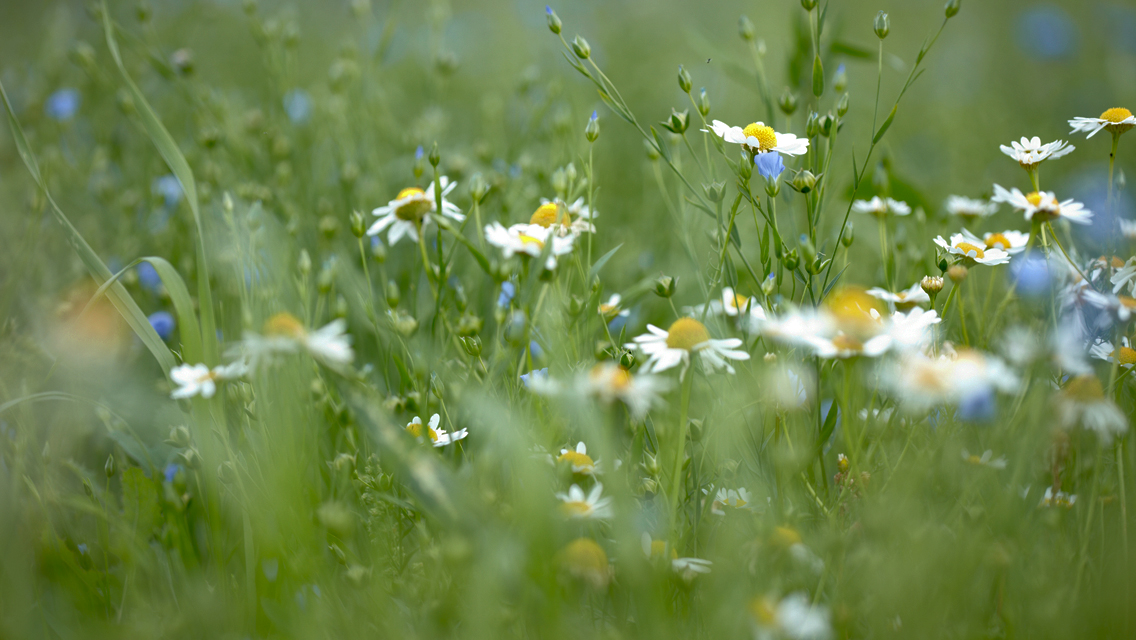
\includegraphics[width=12cm]{Daisy.jpg}| 的命令可以纳入图片.

如图~\ref{fig:1} 是一个纳入~jpg 图片的例子.

\begin{figure}[ht]
\centering
  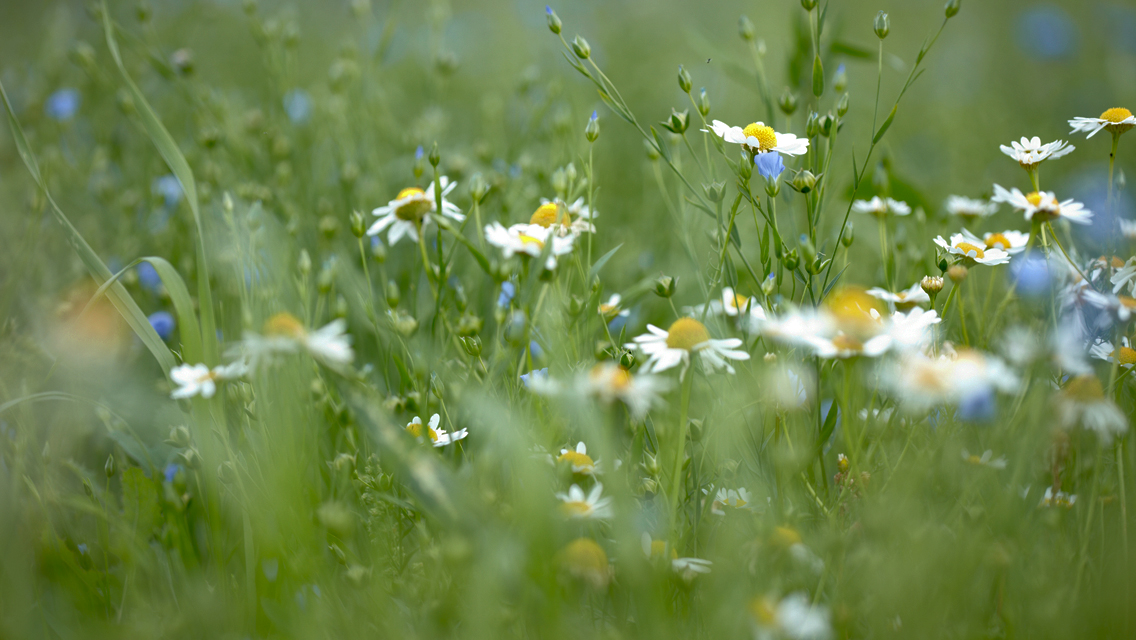
\includegraphics[width=\textwidth]{Daisy.jpg}
  \caption{一个彩色 jpg 图片的例子}
  \label{fig:1}
\end{figure}

表格问题, 建议使用``三线表'', 如表 \ref{tab:1}.

\begin{table}[ht]
\centering
\caption{一般三线表}
\label{tab:1}
    \begin{tabular}{c c c c c c c c c c c}
    \hline
    123 & 4  & 5  & 123 & 4 & 5123 & 4 & 5 & 123 & 4 & 5\\
    \hline
    67 & 890 & 13 & 123 & 4 & 5123 & 4 & 5 & 123 & 4 & 5\\
    67 & 890 & 13 & 123 & 4 & 5123 & 4 & 5 & 123 & 4 & 5\\
    67 & 890 & 13 & 123 & 4 & 5123 & 4 & 5 & 123 & 4 & 5\\
    \hline
    \end{tabular}
\end{table}






%%%%============================================================================================================%%%

\chapter{其他事项}
以下是广告时间, 插播一段广告:
\begin{itemize}
    \item 插图\index{插图}的制作, 建议用 pgf, 也叫 tikz.
          pgf 的长处是源文件直接植入~\TeX~文档, 管理起来非常方便.
    这里有我写的一个关于初次使用~pgf~的帖子:\\    \url{http://bbs.ctex.org/forum.php?mod=viewthread&tid=30480}.
    \item 生成参考文献, 建议使用~BibTeX.\index{BibTeX} 这里有我写的一个文档: \\
    \url{http://bbs.ctex.org/forum.php?mod=viewthread&tid=26056}.

          {\kaishu 使用 BibTeX{} 做参考文献时,
      借助 EndNote 或者 NoteExpress, 可以非常漂亮简单地解决 bib 文件的录入问题.
      NoteExpress 在校图书馆网站有正版软件提供下载.
      当然 EndNote 本身就是 Thomson Corporation 推出的(和 SCI 搜索引擎是同一家公司),
      和多个重要文献搜索引擎有良好的功能配合.

      Google 学术搜索也提供了文献的 bib 格式.
      录入参考文献时, 偶尔用一用 Google 学术搜索, 还可以核查或减少录入的错误, 并减少录入的工作量.}

    \item 幻灯片\index{幻灯片}的制作, 建议使用~Beamer. 这里有我写的一个模板, 谨供参考:\\
    \url{http://bbs.ctex.org/forum.php?mod=viewthread&tid=27695}.
\end{itemize}


%%%============================================================================================================%%%

%%%=== 参考文献 ========%%%
\cleardoublepage\phantomsection
\addcontentsline{toc}{chapter}{参考文献}
\begin{thebibliography}{00}

  \bibitem{r1} 作者. 文章题目 [J].  期刊名, 出版年份,卷号(期数): 起止页码.

  \bibitem{r2} 作者. 书名 [M]. 版次. 出版地:出版单位,出版年份:起止页码.

  \bibitem{r3} 邓建松等, 《\LaTeXe~科技排版指南》, 科学出版社.

  \bibitem{r4} 吴凌云, 《CTeX~FAQ (常见问题集)》, \textit{Version~0.4}, June 21, 2004.

  \bibitem{r5} Herbert Vo\ss, Mathmode, \url{http://www.tex.ac.uk/ctan/info/math/voss/mathmode/Mathmode.pdf}.


\end{thebibliography}

% !Mode:: "TeX:UTF-8"
%%%%%%%%%%%%%%%%%%%%%%%%%%%%-------致谢--------%%%%%%%%%%%%%%%%%%%%%%%%%%%%%%%%

\acknowledgement
\addcontentsline{toc}{chapter}{致谢}


感谢你, 感谢他和她, 感谢大家.











 %%%致谢

%%%-------------- 附录. 不需要可以删除.-----------
\appendix

\chapter{测试}

\section{第一个测试}
测试公式编号
\begin{equation}
1+1=2.
\end{equation}

表格编号测试

\begin{table}[h]
  \centering
  \caption{测试表格}
  \begin{tabular}{*{20}c}
     \hline
     % after \\: \hline or \cline{col1-col2} \cline{col3-col4} ...
     11 & 13  & 13  & 13  & 13 \\
     12 & 14  & 13  & 13  & 13 \\
     \hline
   \end{tabular}
\end{table}


\chapter{附录测试}

测试

\chapter{附录测试}

测试

\cleardoublepage
\end{document}



